\documentclass[11pt,a4paper]{article}
\usepackage{fullpage}
\usepackage[utf8]{inputenc}
\usepackage{anysize}
\usepackage{cite}
\usepackage{graphicx}
\usepackage{fancyhdr}
\usepackage{caption}
\usepackage{algorithm}
\usepackage{hyperref}
\usepackage{listings}
%\usepackage[ngerman]{babel}
\usepackage{subfiles}
\usepackage[T1]{fontenc}
\usepackage[absolute]{textpos}
\usepackage[scaled]{helvet}
\renewcommand{\familydefault}{\sfdefault}
\usepackage{calc} % Calculations
\usepackage{tabto} % Tabs
\usepackage{parskip}
\usepackage{float}

\begin{document}

\marginsize{2.5cm}{3cm}{2.5cm}{2cm}
\makeatletter
\def\ps@myPS{%
    \def\@oddfoot{\null\hfill\thepage}
    \def\@evenfoot{\thepage}%
    \def\@evenhead{\null\hfil\slshape\leftmark}%
    \def\@oddhead{{\slshape\rightmark}}}%
\makeatother
\pagestyle{myPS}

\author{\textbf{Gregor Ziegltrum, Martin Bogusz, Sven Schepp}}
\title{\textbf{Wave-Propagation-Simulator}}
\maketitle
\linespread{1.8}

\begin{center}
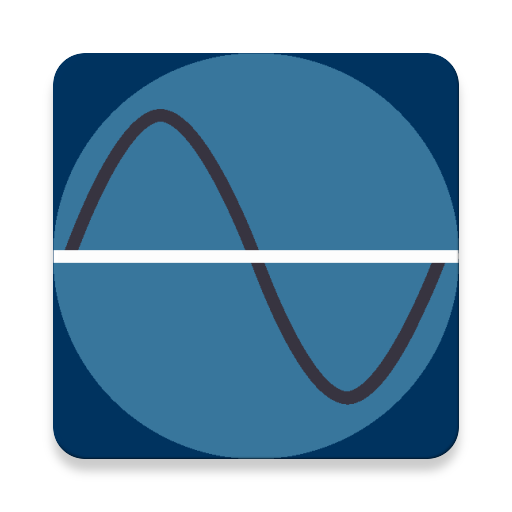
\includegraphics[scale=0.30]{ic_launcher-web.png}
\end{center}



\pagebreak
\thispagestyle{empty}
\tableofcontents
\pagebreak


\section{Introduction}

This project was designed to allow for simple wave-obstacle-interaction-simulation to be ported onto mobile Android-Systems. It entails adding waves onto a domain of calm water to simulate the effects of tsunamis. Additionally, the user is able to add landmasses to the domain and imitate the behavior of waves interacting with various shapes. Reflecting boundary conditions are an optional feature, enclosing the domain within surrounding terrain. The application is available to be used on all Android devices with API level 22 or higher and can be tested on any desktop through the Android Studio development environment.


\begin{figure}[H]
\begin{center}
\vspace{3cm}
\includegraphics[scale= 1]{DefaultView.png}
\caption{Default view}
\end{center}
\end{figure}







\pagebreak
\section{Features}
All the previously mentioned features, will be presented in further detail in the next subsections.

\subsection{Waves}
The user can simulate simple waves by tapping the blue domain on the screen.


\begin{figure}[H]
\makebox[\textwidth]{%
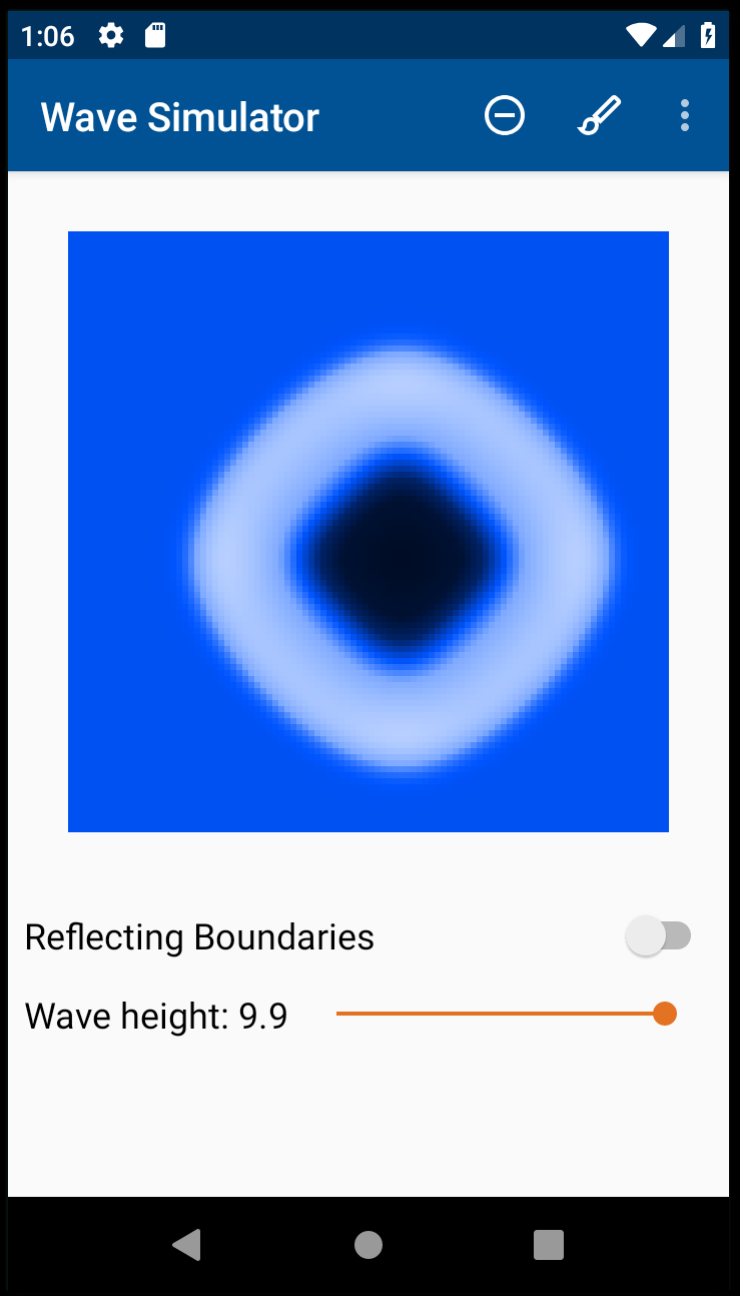
\includegraphics[width=0.49\textwidth]{Wave.png}%
\hfill    
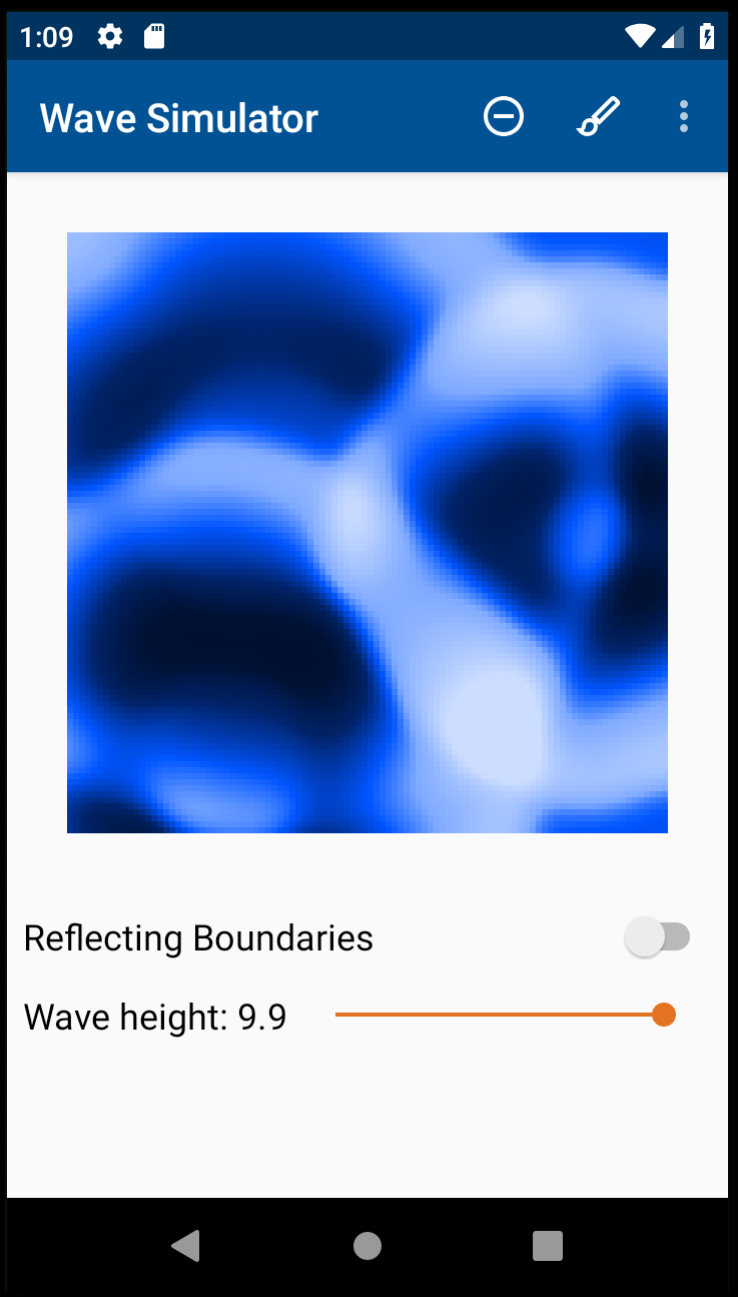
\includegraphics[width=0.49\textwidth]{Waves.png}%
}
\caption{Height slider in orange}
\end{figure}





The height of the waves is adjustable through the orange slider below the domain. The maximum height of 9.9 is set as the default option. The minimum is set to be 5.0. Tapping the screen multiple times will add a wave for every tap performed and its height will be determined by the current status of the slider. The simulation will be automatically halted if only very little wave-movement is detected.

\subsection{Obstacles}
The user can define obstacles inside the given domain. They are made visible in green. Any given shape can be produced by sliding the finger across the domain.


\begin{figure}[h]
\makebox[\textwidth]{%
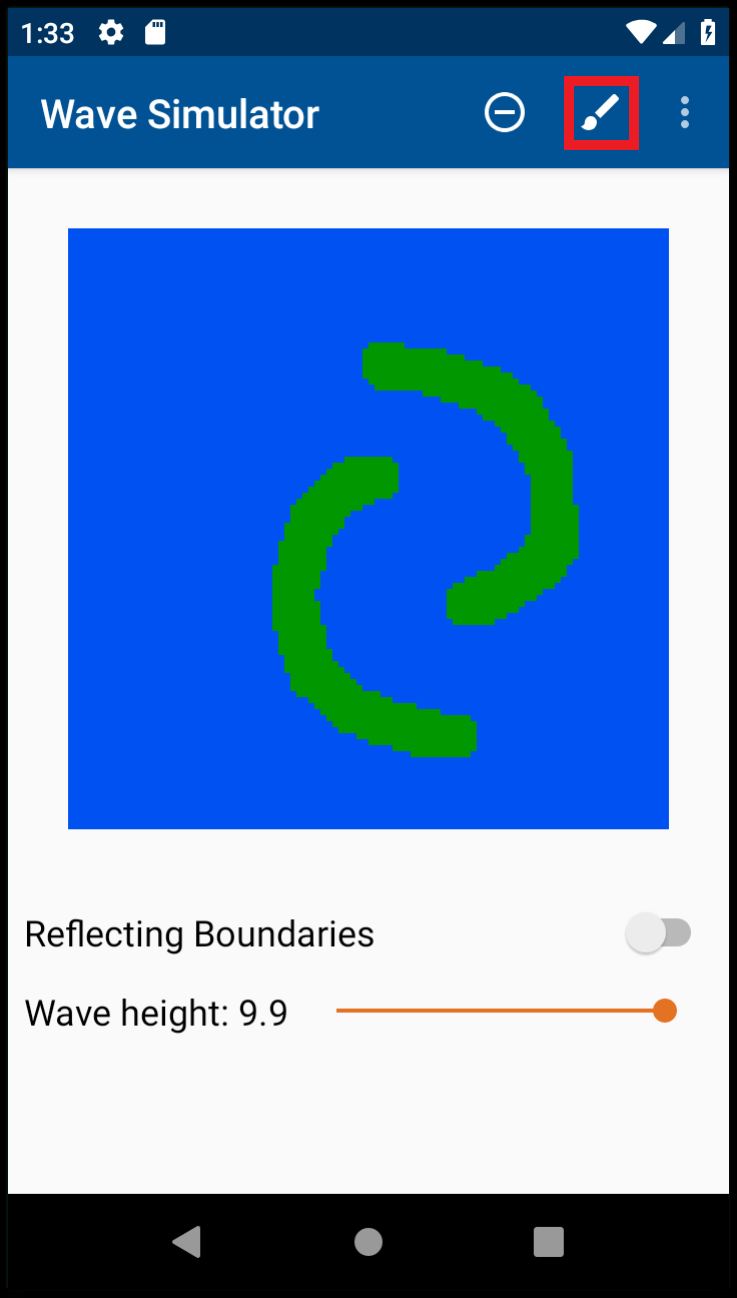
\includegraphics[width=0.49\textwidth]{Obstacle.png}%
\hfill    
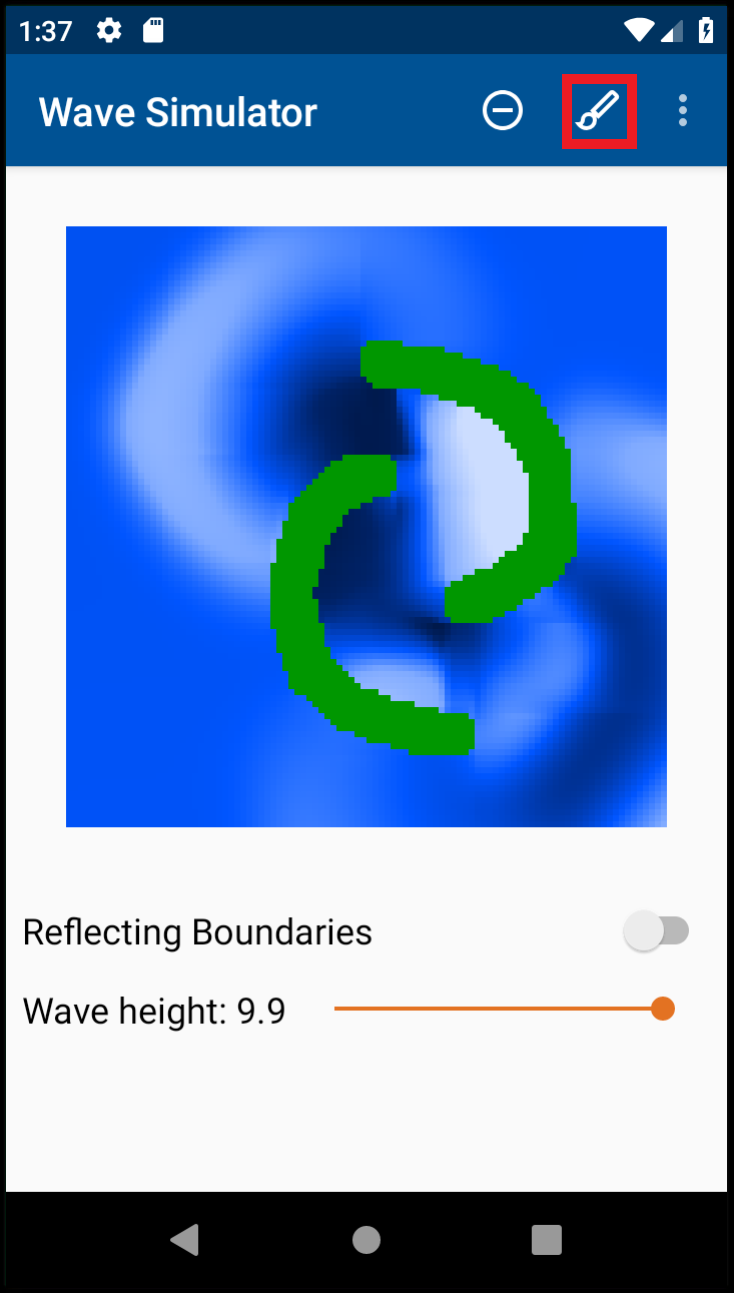
\includegraphics[width=0.49\textwidth]{ObstacleW.png}%
}
\caption{Brush-Symbol marked red}
\end{figure}


If the user adds  waves to a modified domain, the waves will interact with the drawn environment.  The user has to select the 'brush' icon in the top left corner of the screen to  enter 'draw' mode. The user will be reminded of this by a message on the bottom of the screen in addition to the brush icon changing to a completely white version. As long as the user stays in 'draw' mode, no waves can be set. The user can leave the 'draw' mode via the brush icon. The user will be reminded once again by a message and the icon changing back to its former look.


\pagebreak
\subsection{Boundary Conditions}
The option to change the boundary conditions from 'outflow' to 'reflecting' can be found directly below the domain. While the former option results in the wave flowing out of the domain, the latter allows the waves to bounce back into it. The default option is set to be 'outflow'.

\begin{figure}[H]
\vspace{2cm}
\makebox[\textwidth]{%
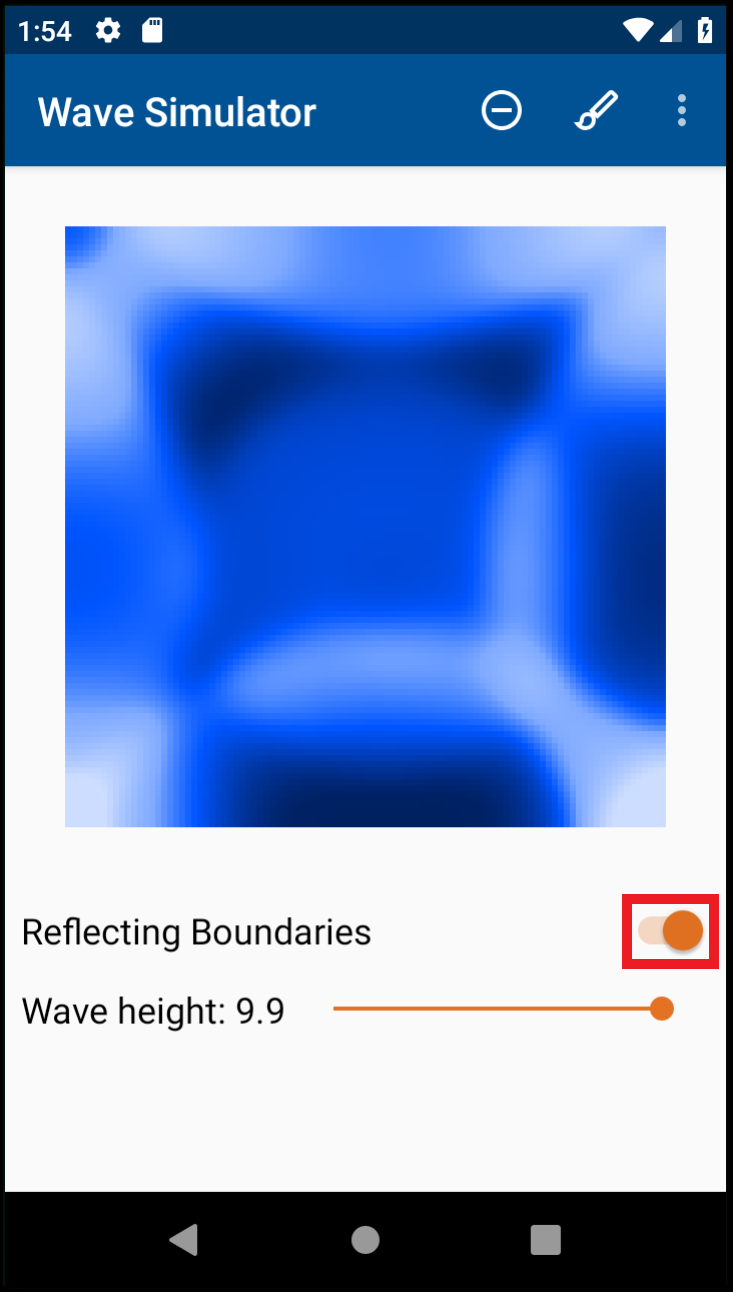
\includegraphics[width=0.49\textwidth]{Boundary.png}%
\hfill    
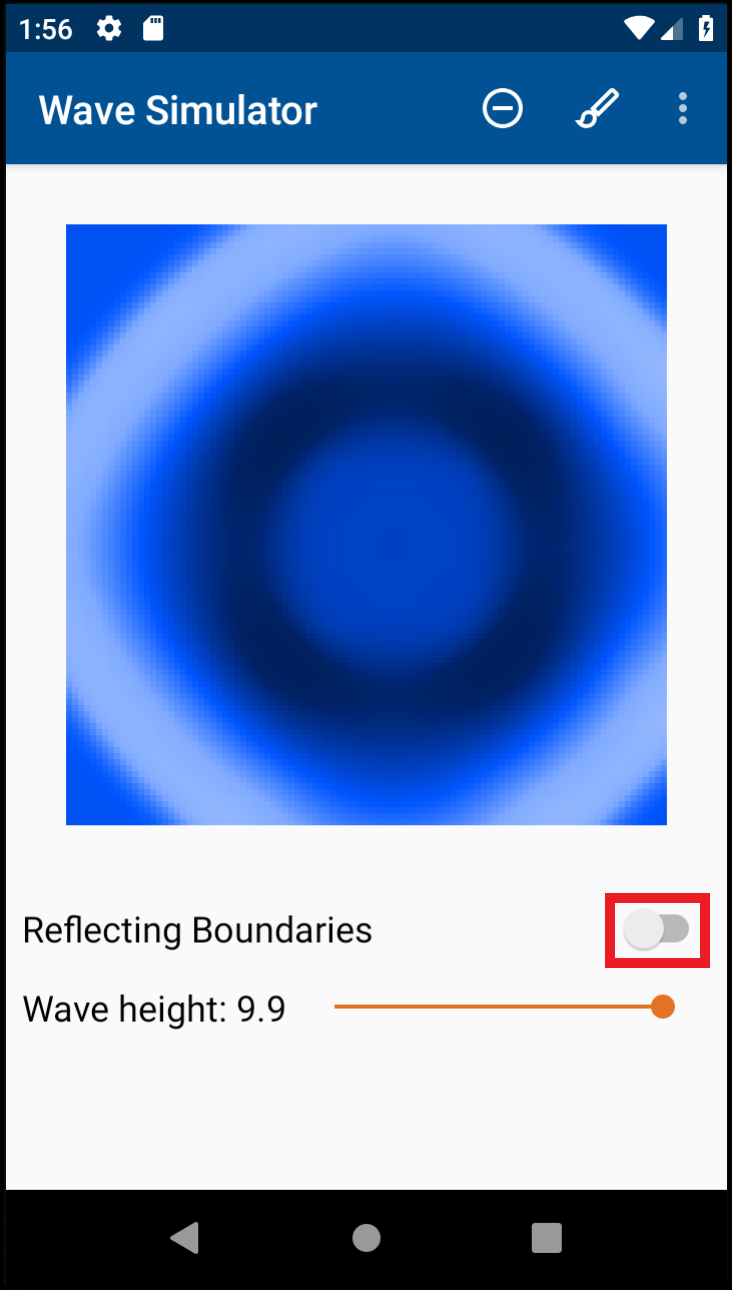
\includegraphics[width=0.49\textwidth]{NoBoundary.png}%
}
\caption{Reflecting boundary-conditions are enabled in the left figure. Switch marked in red.}
\end{figure}

\pagebreak
\subsection{Erasing}
To erase a part of the drawn bathymetry, the user has enter 'erase' mode by tapping the minus icon in the top middle of the screen. The user will be reminded of having entered the 'erase' mode by a message on the bottom of the screen as well as the minus icon changing to the inverted version. Removing the obstacles is done in the same way as adding them, by swiping over them. No waves can be set in this mode.

\begin{figure}[H]
\vspace{2cm}
\makebox[\textwidth]{%
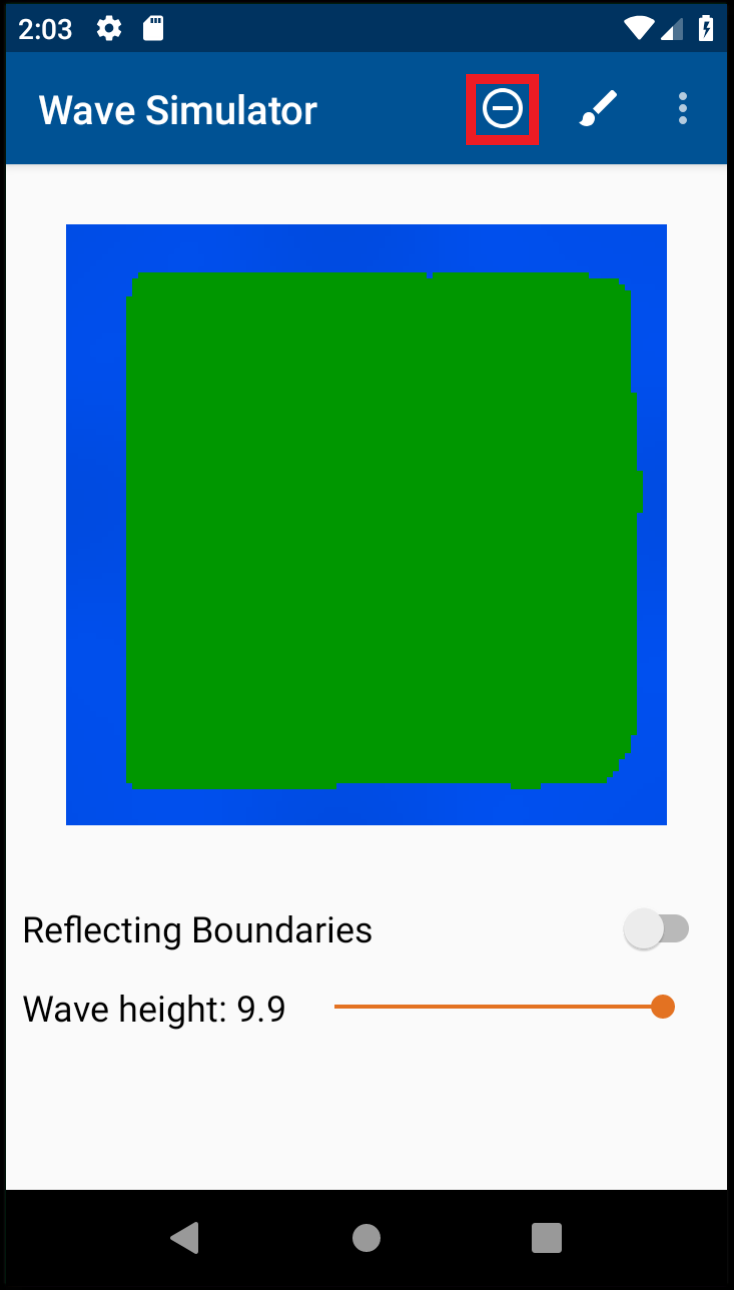
\includegraphics[width=0.49\textwidth]{NoErasure.png}%
\hfill    
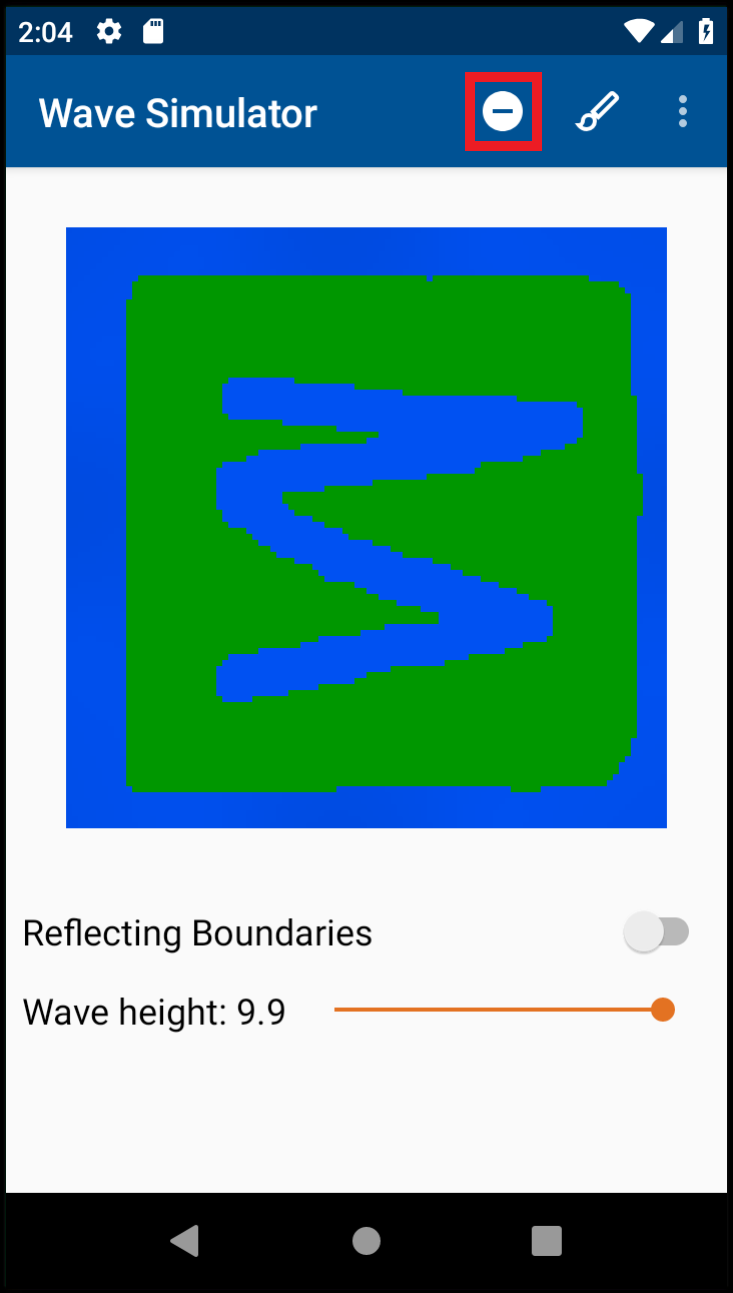
\includegraphics[width=0.49\textwidth]{Erasure.png}%
}
\caption{
The bathymetry drawn on the left has been modified in the right figure.
Minus-icon marked in red.
}
\end{figure}


\subsection{Resetting}
The user can choose to reset the entire domain, or just the waves. This is done by selecting the options icon on the top most left corner of the screen and choosing the respective option. After tapping the desired option, a reset will occur and the user can continue to use the app without any further action.

\begin{figure}[H]
\vspace{2cm}
\makebox[\textwidth]{%
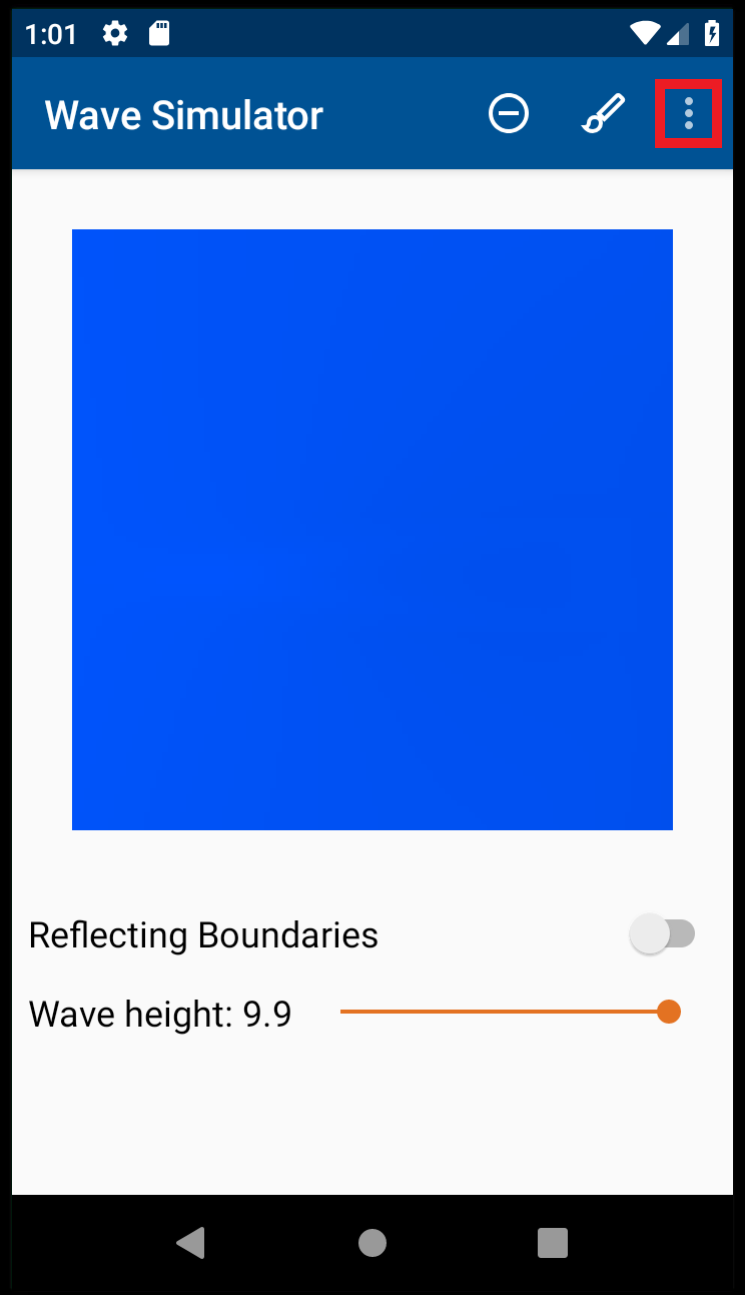
\includegraphics[width=0.49\textwidth]{ResetI.png}%
\hfill    
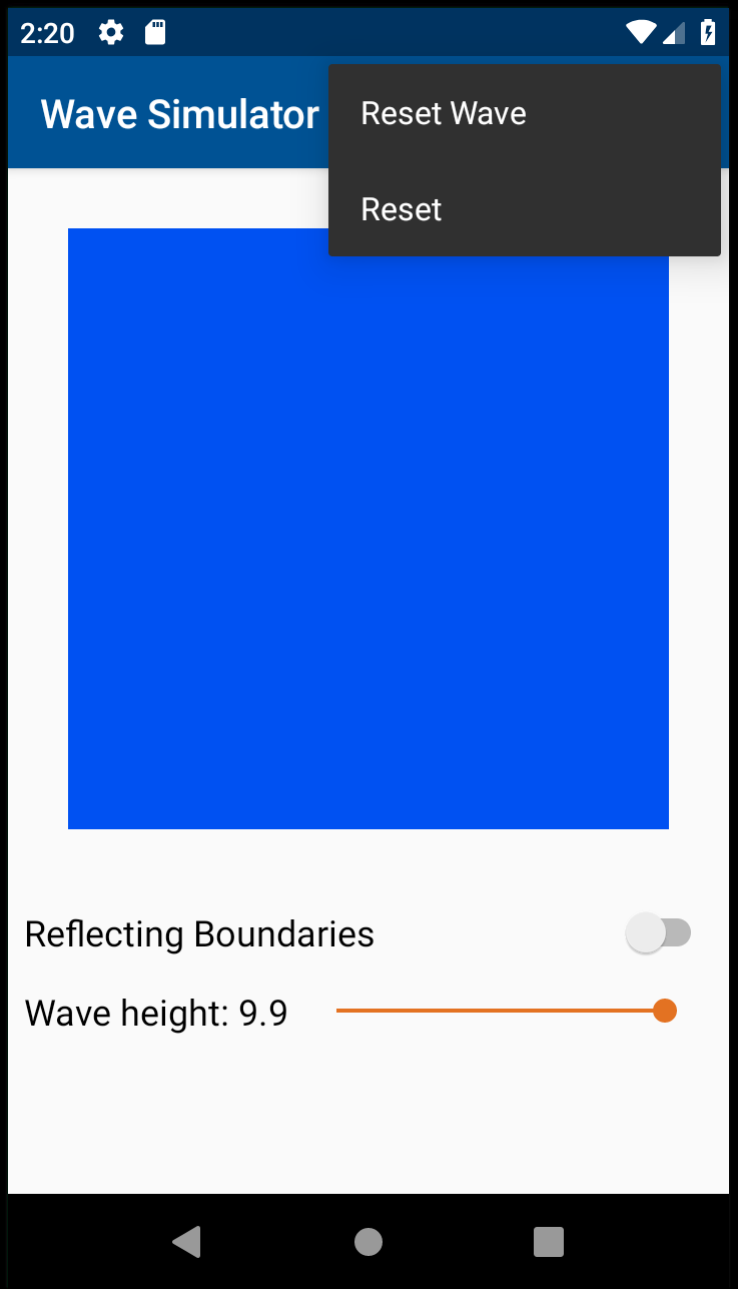
\includegraphics[width=0.49\textwidth]{ResetS.png}%
}
\caption{Reset options shown right. Options symbol highlighted in red on the left}
\end{figure}

\pagebreak


\section{Examples}
%These are a few examples that showcase the apps functionalities.

\begin{figure}[H]
\makebox[\textwidth]{%
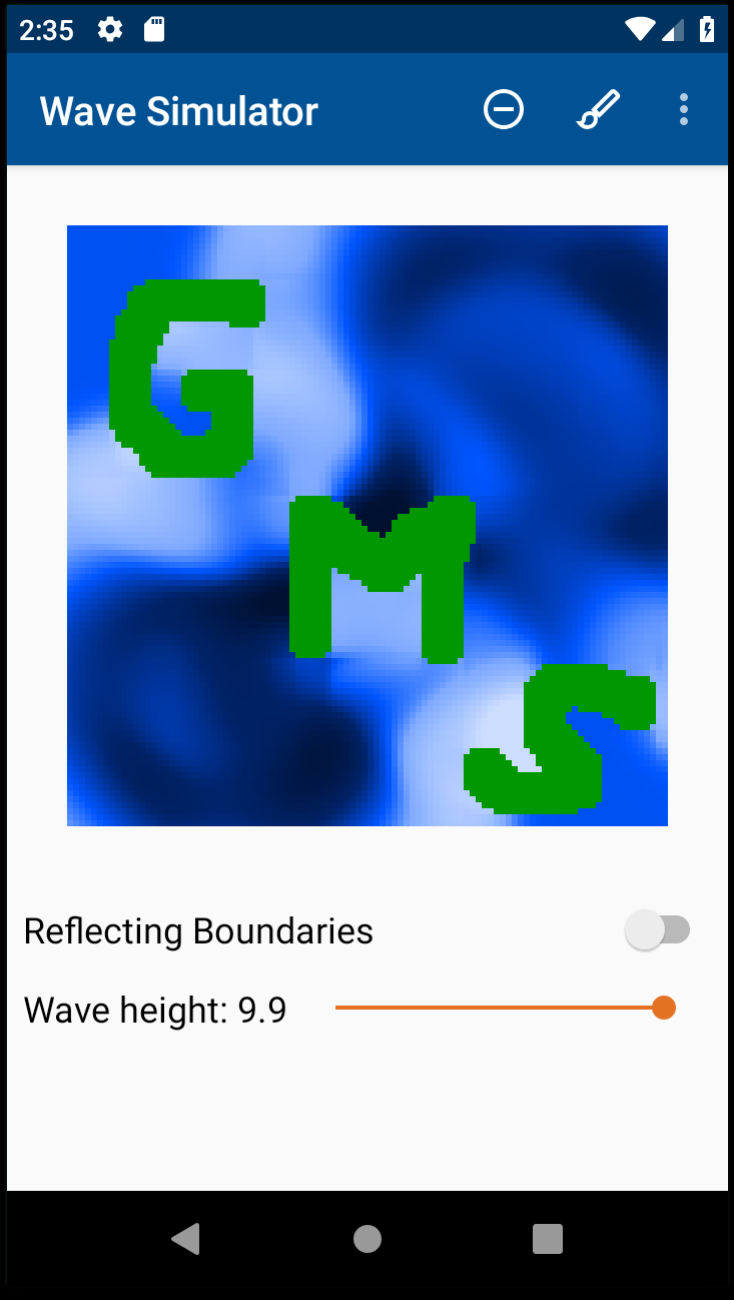
\includegraphics[width=0.45\textwidth , height = 10.5cm]{GMS.png}%
\hfill    
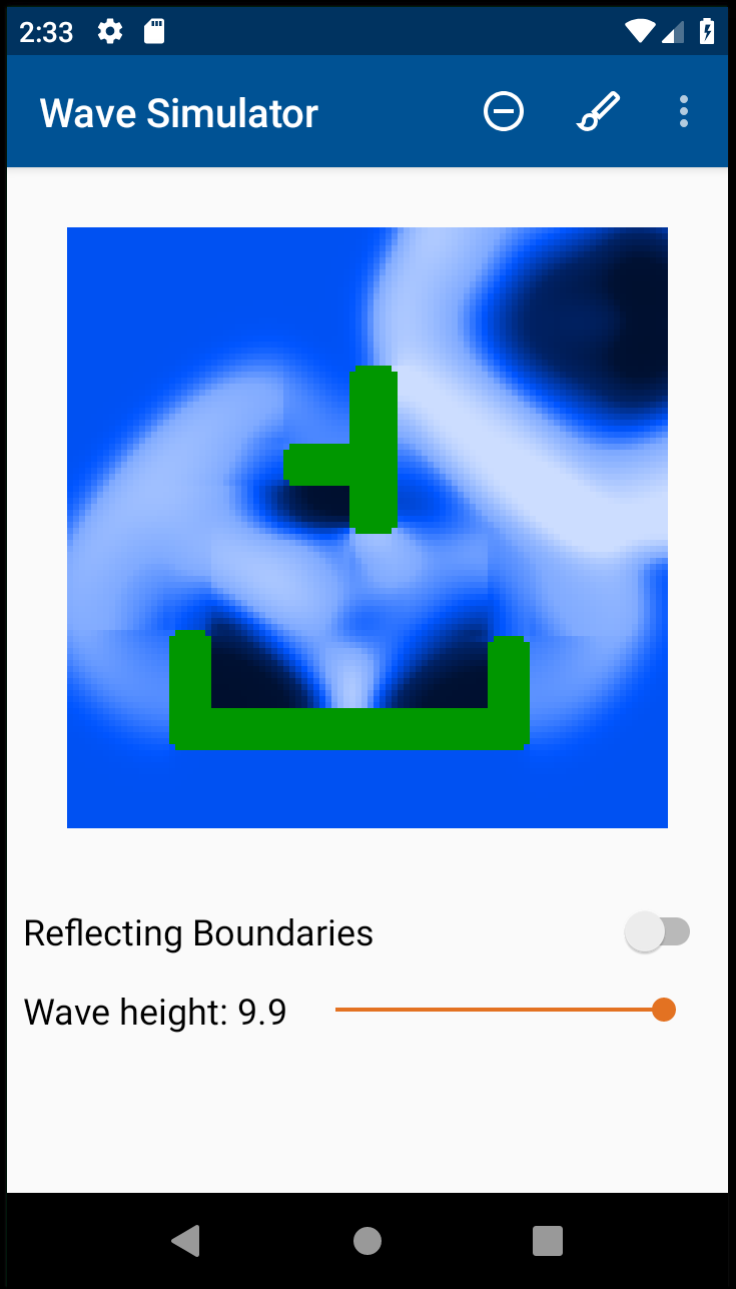
\includegraphics[width=0.45\textwidth , height = 10.5cm]{TU.png}%
}\vspace{0.25cm}
\makebox[\textwidth]{%
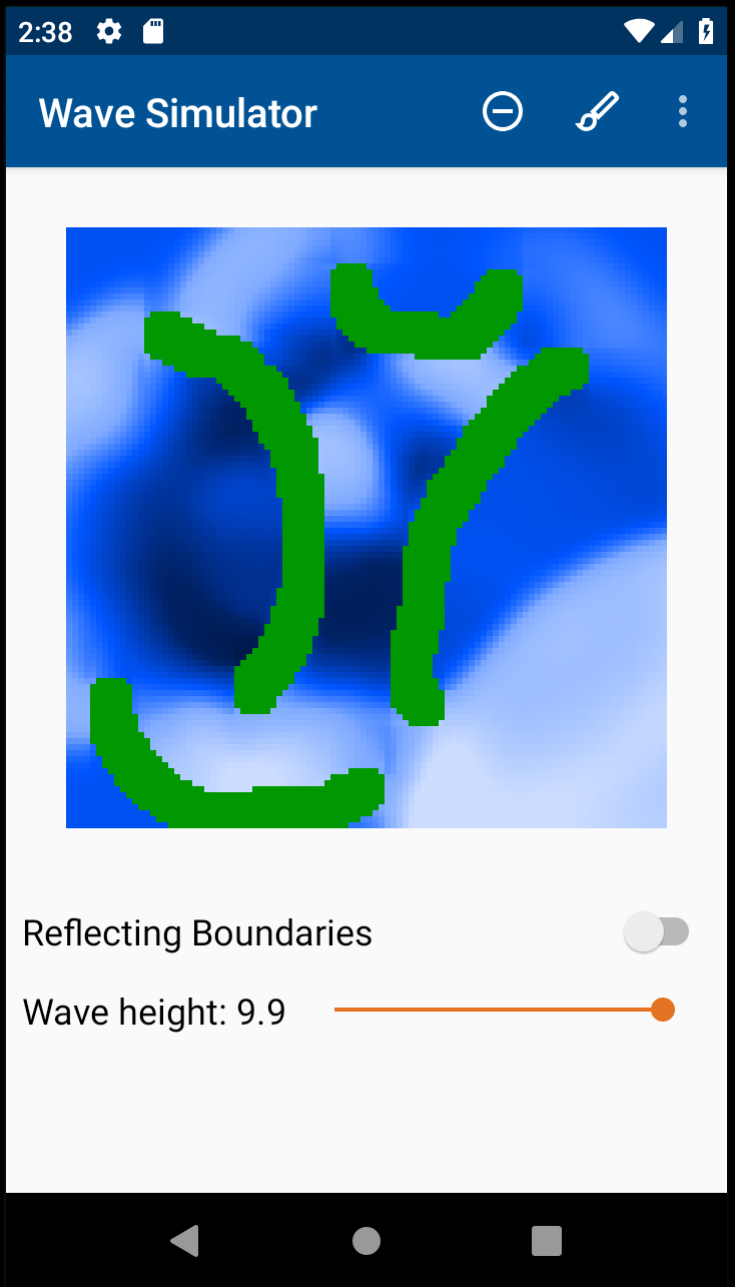
\includegraphics[width=0.45\textwidth , height = 10.5cm]{Swung.png}%
\hfill    
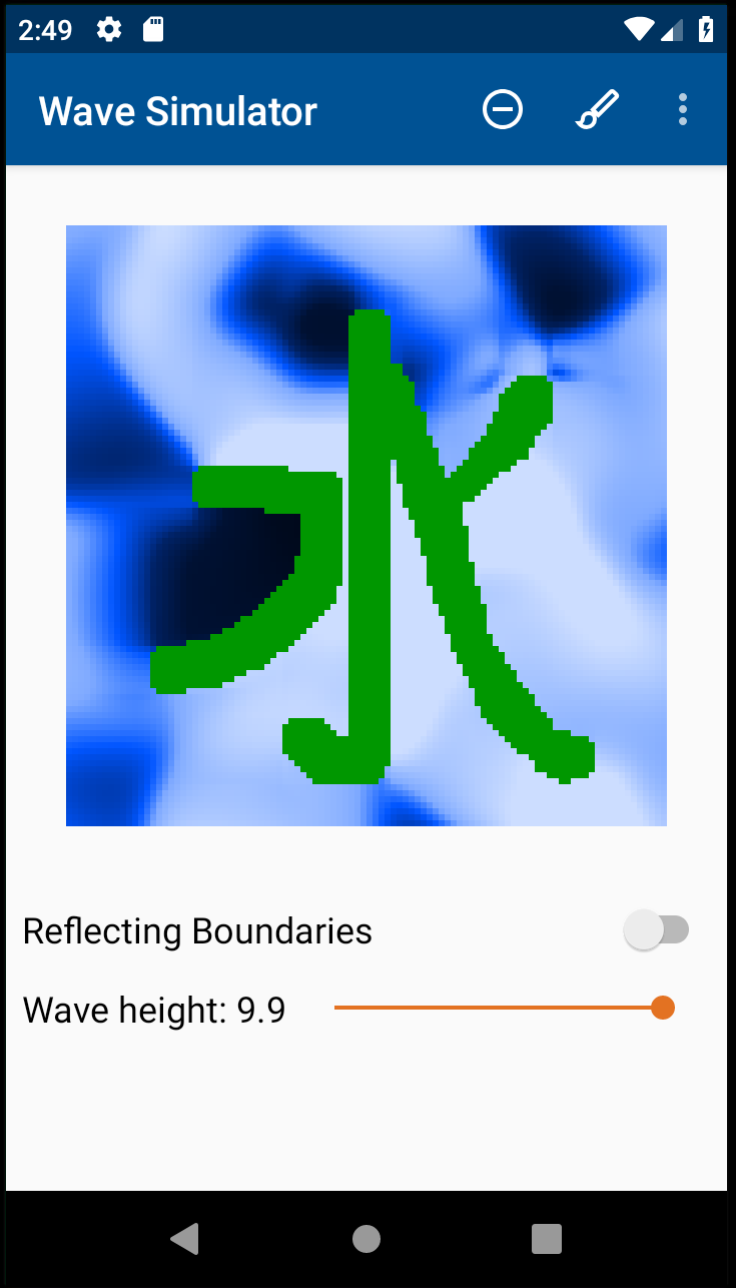
\includegraphics[width=0.45\textwidth , height = 10.5cm]{Mizu.png}%
}
\caption{Examples presented by our team}
\end{figure}

\pagebreak
\section{Accessing the Application}
Our app can be downloaded from the \href{https://play.google.com/store/apps/details?id=gregor.wavesimulator}{Google-Play-Store}.
The code for the application can be found in our \href{https://gitlab.lrz.de/ga84niv/WaveSimulator.git}{git-repository} and has to be executed via \href{https://developer.android.com/studio/}{Android Studio}. It is sufficient to only open the 'app' folder of our project. All prerequisites needed for running the app on a desktop or an Android-device\footnote{To run simulations on external Android devices, \href{https://developer.android.com/studio/run/oem-usb}{installing OEM USB-drivers} is necessary} is detailed on the Andriod Studio website. To run the app on a real Android device, developer mode has to be enabled. 

\end{document}